\section*{Änderungshistorie}
%Textbreite 14cm
\begin{longtable}{|p{2cm}|p{2cm}|p{3cm}|p{7cm}|} \hline
	
	\textbf{Version} & \textbf{Datum} & \textbf{Autor} & \textbf{Beschreibung}\\ 
	\begin{tabularx}{\textwidth}{|l|X|}{
			\hline
			Aufwand & [50]{h} \\\hline
			Personen & Daniel Zimmermann \\\hline
			Arbeitsmittel & Ergebnisse von \ref{sec:info} und \ref{sec:Konzeptphase} \\\hline
			Ergebnisse &  komplettes Produkt zum Test bereit\\\hline
		\end{tabularx}
		
		\subsection{Testphase}
		\label{sec:test}
		Dieses Arbeitspaket umfasst den Test der entwickelten Hard- und Software.
		Es werden zunächst die mechanischen Tests durchgeführt, danach  werden softwaresetige Tests getätigt.
		Anschließend findet der Test auf dem Packbot statt. Diese Phase umfasst auch die Behebung der festgestellten Mängel. \\
		
		\begin{tabularx}{\textwidth}{|l|X|}
			\hline
			Aufwand & [20]{h} \\\hline
			Personen & Daniel Zimmermann\\\hline
			Arbeitsmittel & Ergebnisse von \ref{sec:real}, Laborgeräte, Packbot\\\hline
			Ergebnisse & Dokumentation der Testergebnisse, Fehlerbereinigte Hard-/Software, Liste der verbleibenden Mängel \\\hline
		\end{tabularx}
		
		\subsection{Dokumentation}
		\label{sec:doku}
		Dieses Arbeitspaket umfasst die gesamte Erstellung der Projektdokumentation. Das beinhaltet die gesamten Vorgaben, welche in den Anforderungen protokolliert sind. Es werden Ergebnisse aus den verschiedenen Phasen detailliert präsentiert und entsprechende Erläuterungen zu Problemstellungen und Vorgehensweisen gemacht. Jedes Unterkapitel wird reflektiert. \\
		
		\begin{tabularx}{\textwidth}{|l|X|}
			\hline
			Aufwand & [100]{h} \\\hline
			Personen & Daniel Zimmermann \\\hline
			Arbeitsmittel & Latex, Word, Excel \\\hline
			Ergebnisse & Projektdokumentation, Projektmanagement, Schlussbericht,  \\\hline
		\end{tabularx}
		
		\subsection{Präsentation \& Poster}
		\label{sec:Pras}
		Dieses Arbeitspaket beinhaltet alle Phasen der Präsentation.  Es wurden somit das Erstellen und Abhalten der Zwischenpräsentation, der Abschlusspräsentation und des Posters zusammengetragen.   \\
		\begin{tabularx}{\textwidth}{|l|X|}
			\hline
			Aufwand & [25]{h} \\\hline
			Personen & Daniel Zimmermann \\\hline
			Arbeitsmittel & Powerpoint, Bericht \\\hline
			Ergebnisse & Zwischenpräsentation, Abschlusspräsentation, Poster  \\\hline
		\end{tabularx}
		
		
		\subsection{Präsentation \& Poster}
		\label{sec:Praesi}
		Dieses Arbeitspaket beinhaltet alle Phasen der Präsentation.  Es wurden somit das Erstellen und Abhalten der Zwischenpräsentation, der Abschlusspräsentation und des Posters zusammengetragen.   \\
		\begin{tabularx}{\textwidth}{|l|X|}
			\hline
			Aufwand & [25]{h} \\\hline
			Personen & Daniel Zimmermann \\\hline
			Arbeitsmittel & Powerpoint, Bericht \\\hline
			Ergebnisse & Zwischenpräsentation, Abschlusspräsentation, Poster  \\\hline
		\end{tabularx}
		
		
		
		%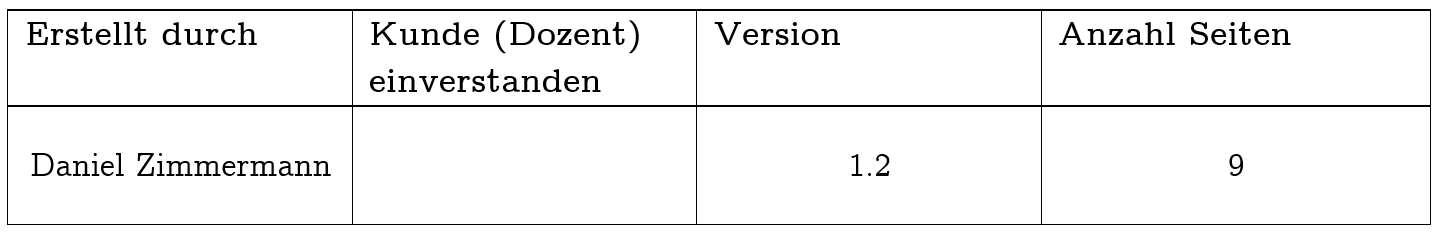
\includegraphics[width=1 \textwidth]{bilder/Pflichtenheft_6.PNG}
		
	
	1.0 & 03.10.2017 & D. Zimmermann & Erstellung\\

	
\end{longtable}